\chapter{Ala}
Començant pels càlculs més bàsics, s'estudia el comportament de l'ala com a cos aïllat.

\section{Angle de sustentació nul·la}
L'únic paràmetre geomètric de l'ala que queda per determinar és l'angle de twist. Per tal de fer-ho, és útil calcular l'angle de sustentació nul·la de la secció central de l'ala per a diferents valors d'aquest angle, concretament en el rang de -8 a 0$^{\circ}$.

\begin{figure}[h]
	\centering
	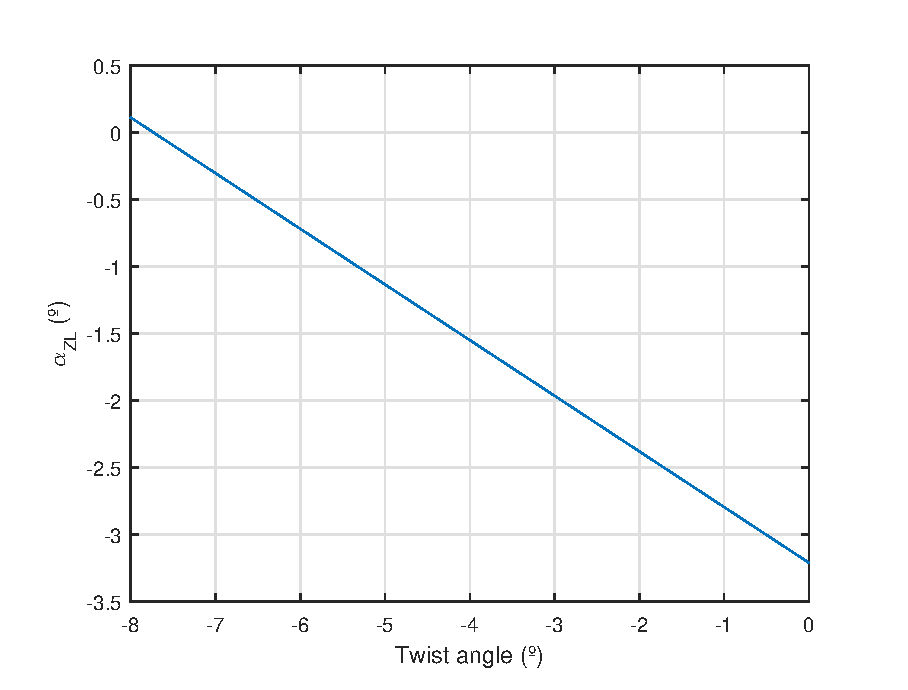
\includegraphics{./plots/zlangle}
	\caption{Angle de sustentació nul·la per diferents valors de twist}
	\label{zla}
\end{figure}

Els resultats d'aquest estudi es resumeixen en la figura \ref{zla}. Com es pot observar, la dependència entre l'angle de twist i l'angle de sustentació nul·la és completament lineal. A mesura que el twist es torna més negatiu, l'angle de sustentació nul·la augmenta.

Tenint en compte aquests resultats, es determina que per a tal de tenir el màxim de sustentació possible, el millor angle de twist és el que permet un angle de sustentació nul·la més baix. Per tant, s'escull un twist de $\theta=0^{\circ}$.

\section{Resistència aerodinàmica}
A l'hora de calcular l'angle de sustentació nul·la per a diferents valors de twist, també s'ha determinat el coeficient de resistència aerodinàmica total.

Com és de suposar, ja que la sustentació és nul·la, la resistència induïda també és nul·la. No obstant, cal tenir en compte la resistència paràsita. Aquesta, com s'observa a la figura \ref{cdpar}, no depèn de l'angle de twist, ja que no depèn de la sustentació, i pren un valor constant de $C_{D}=C_{D_{0}}=0.0063$.

\begin{figure}[h]
	\centering
	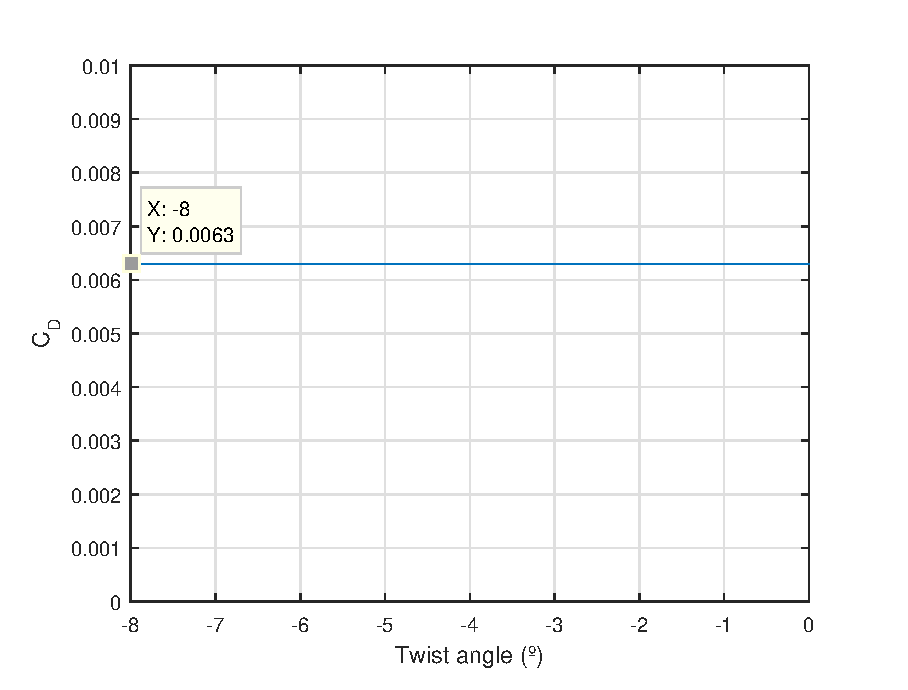
\includegraphics{./plots/cdparasita}
	\caption{Resistència aerodinàmica en angle de sustentació nul·la}
	\label{cdpar}
\end{figure}

\section{Corba polar}
Finalment, per completar l'anàlisi de l'aerodinàmica de l'ala, és necessari calcular els coeficients de sustentació i de resistència aerodinàmica. Per tal d'obtindre diversos valors significatius, aquests s'estudien per a diversos angles d'atac, de 0 a 10$^{\circ}$.

\begin{figure}[h]
	\centering
	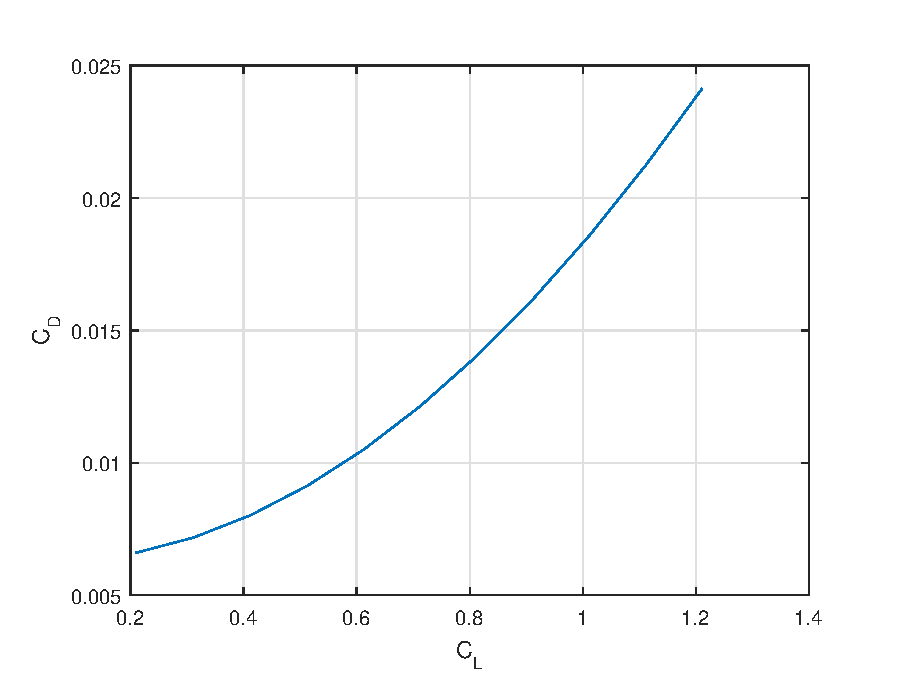
\includegraphics{./plots/polarcurve}
	\caption{Corba polar ($C_{D}$ vs. $C_{L}$)}
	\label{polar}
\end{figure}

Com s'observa a la figura \ref{polar}, la representació gràfica del coeficient de resistència aerodinàmica en funció del coeficient de sustentació pren forma de paràbola, tal i com s'esperava.